%---------------------
% START OF PREAMBLE - do not delete!
%---------------------
\documentclass[12pt]{article}
\usepackage[pdftex]{graphicx}
\usepackage{amsmath}
\usepackage{verbatim}
\DeclareGraphicsRule{*}{mps}{*}{}

%==============================================================================
% Page layout
%==============================================================================

%------------------------------------------------------------------------------
%  Define the page dimensions.
%------------------------------------------------------------------------------
\setlength{\hoffset}{0.0in}
\setlength{\oddsidemargin}{0.0in}
\setlength{\evensidemargin}{0.0in}
\setlength{\textwidth}{6.75in}

\setlength{\voffset}{0in}
\setlength{\topmargin}{-.6in}
\setlength{\headheight}{12pt}
\setlength{\headsep}{12pt}
\setlength{\textheight}{9.5in}
\renewcommand{\baselinestretch}{1.0}
\renewcommand{\labelitemi}{-}

% writing the section number and the subsection number together
% and also the subsubsection in the form of 1.a
\renewcommand\thesubsection{\arabic{section}.\alph{subsection}}
\renewcommand\thesection{Problem \arabic{section}}
%------------------------------------------------------------------------------

%---------------------
% END OF PREAMBLE - do not delete!
%---------------------

\begin{document}

%---------------------
% make the title
%---------------------
\title{Homework 3}
\author{Masoud Akbarzadeh}
\date{\today}

\maketitle
% make these as info on top of the page
\begin{center}
    {\bf Estimated time to Completion}: {10 hours} \\
    {\bf Maximum Allocated Time}: {15 hours} \\
    {\bf Actual Time to Completion}: {11 hours} \\
    {\bf Collaborators}: {Nari, Juan, Amel, Brandon, Jennifer, Kat, Bali, Chelsea,Jesse, Katurah, Delian} \\

\end{center}
%\newpage
%---------------------

%---------------------
% begin main text
%---------------------
\section{}\label{sec:problem-1}
\subsection{}\label{subsec:problem-1-a}

\begin{figure}
\begin{center}
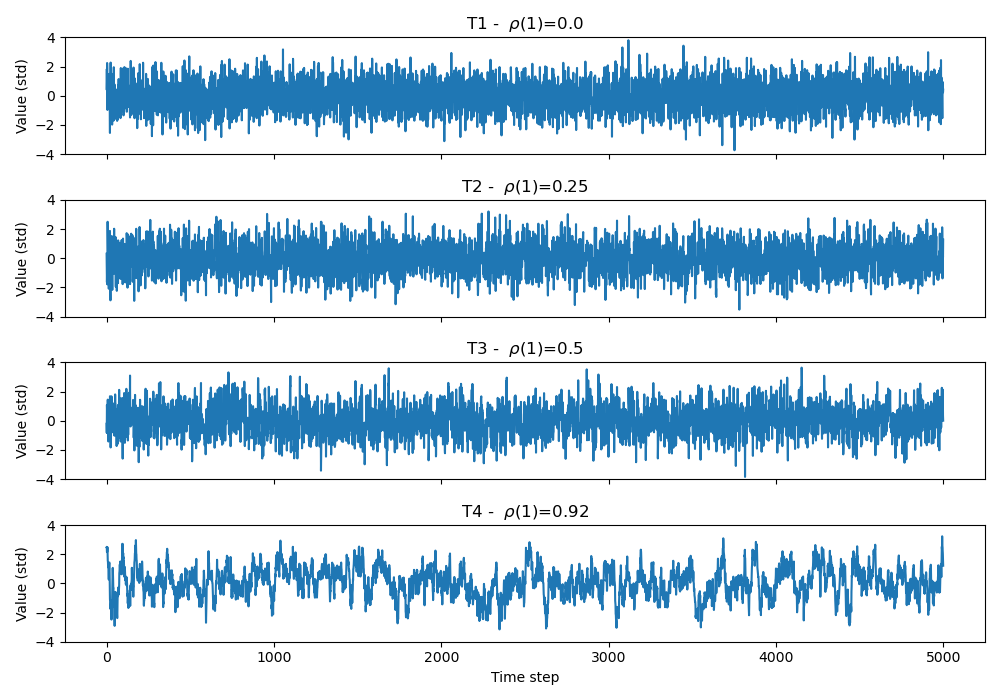
\includegraphics[width=6in]{p1_1_hw1_red_noise_time_series.png}
\caption{Problem 1 - Plots of each time series}{\label{fig:problem-1-a}}
\end{center}
\end{figure}


\begin{figure}
\begin{center}
\includegraphics[width=6in]{p1_2_hw1_hist_sample_mean_all.png}
\caption{Problem 1 - Plots all sample means of 100 consecutive samples}{\label{fig:problem-1-a}}
\end{center}
\end{figure}


\begin{figure}
\begin{center}
\includegraphics[width=6in]{p1_2_hw1_hist_sample_std_all.png}
\caption{Problem 1 - Plots all sample standard devation of 100 consecutive samples}{\label{fig:problem-1-a}}
\end{center}
\end{figure}


\subsection{}\label{subsec:problem-1-b}

\subsection{}\label{subsec:problem-1-b}
All the sample means are around zero.
However, the mean values for timeseries with higher lag the mean values has higher spread.
This is because when the lag is higher in other words it means that the $N^*$ is considerably smaller so the spread of the means should be higher.
Also when we grab a sample from a time series with a higher lag, the values are close to the first sample, so our mean is prestty close to the first sample.
\\
Generally the standard deviation of the sample means is around 1. However, the standard deviation of the sample means decreases as the lag increases.
This is because the samples with higher autocorrelation have less variance and the sample means are more consistent.



\\ Assumptions:
\begin{itemize}
    \item Confidence level: 95\% (two-tailed)
    \item $H_0: \mu = 846.33$
    \item $H_1: \mu \neq 846.33$
    \item Z-critical value: 1.96
\end{itemize}
\[ Z = \frac{\=X-\mu}{S / \sqrt{N}} = \frac{847.03-846.33}{5.62/\sqrt{384}} = 2.44 > 1.96 \] \\
Since the z-score is greater than the critical value, the null hypothesis is rejected.
So the average pressure when it rains is significantly different from the average pressure.

\subsection{}\label{subsec:problem-1-c}
Using bootstrapping, 100000 samples were generated.
By calculating the fraction of the time the average pressure when it rains is greater than the average pressure, the p-value was calculated to be 0.007.
So the likelihood of the average pressure being greater when it rains is about 0.7\%.
So the results is in agreement with the z-test.\\
Since the number of data points is large enough, the central limit theorem applies, and the distribution of the sample means is approximately normal.
So using the z-test is valid.\\
\\

\begin{figure}
\begin{center}
\includegraphics[width=5in]{problem1-partA.png}
\caption{Problem 1-A}
\end{center}
\end{figure}

\begin{figure}
\begin{center}
\includegraphics[width=5in]{problem1-partC.png}
\caption{Problem 1-C}
\end{center}
\end{figure}

%new page
\newpage
\section{}\label{sec:problem-2}
% part A of problem 2 % subsection written in form of 2.a
\subsection{Hypothesis testing}\label{subsec:problem-2-a}
Hypothesis testing with these assumptions:
    % bullet points
    \begin{itemize}
        \item # $H_0: \mu = 0$
        \item Two-tailed confidence interval of 95\%
        \item Using z-score since the sample size is larger than 30
        \item A two-tailed test is used
        \item Z-critical value is 1.96
        \end{itemize}

\[ Z = \frac{\=X-\mu}{S / \sqrt{N}} = \frac{0.13-0}{1/\sqrt{100}} = 1.3 < 1.96 \] \\

So we cannot reject the null hypothesis that the air is from the west.
\subsection{Bayesian Approach}\label{subsec:problem-2-b}
Assuming:
\begin{itemize}
    \item $\gamma = 0.4$ is the fraction of time the wind is from the east, and $\gamma = 0.6$ is the fraction of time the wind is from the west
    \item Calculating the probability of the concentration of a pollutant being between 0.12 and 0.14 instead of exactly 0.13
\end{itemize}
Using Bayes' theorem:
\begin{gather*}
    Pr(W) = 0.4\\
    Pr(\=W) = 0.6\\
    Pr(0.12<\=C_{100}<0.14|W) = 0.034\\
    Pr(0.12<\=C_{100}<0.14|\=W) = 0.062\\
    Pr(W|0.12<\=C_{100}<0.14)=\frac{Pr(0.12<\=C_{100}<0.14)Pr(W)}{Pr(0.12<\=C_{100}<0.14)Pr(W)+Pr(0.12<\=C_{100}<0.14|\=W)Pr(\=W)}\\
    Pr(W|0.12<\=C_{100}<0.14)=0.268 < 0.5\\
\end{gather*}
Because $Pr(W|0.12<\=C_{100}<0.14)<0.5$ this approach says the wind is from the east.
\nextpage
\subsection{Sensitivity Analysis}\label{subsec:problem-2-c}

Assuming $\gamma$ values are from $0$ to $1$.
For each of gamma, 10000 monte carlo simulations were run.
Then the fraction of time each approach gives the correct answer was calculated.
The results are shown in the figure ~\ref{fig:problem-2-c}.\\
The results show that for all values of $\gamma$, the Bayesian approach is better than the hypothesis testing approach for this problem.
This is because the Bayesian approach is using the prior information about the wind direction.
Also, the Bayesian approach is least effective when $\gamma = 0.5$ while the frequentist approach is least effective when $\gamma = 0$.
The model in the frequentist approach does not have any knowledge about the wind that is coming from the east, and its probability of happening so the model is only effective in $\gamma$ values close to 1 where the most probable wind is from the west.


\begin{figure}\label{fig:problem-2-c}
\begin{center}
\includegraphics[width=5in]{problem2-partC.png}
\caption{Problem 2-C}
\end{center}
\end{figure}
    \item

\end{document}


